% Preamble
\documentclass[tikz,border=12pt,12pt]{standalone}
\usepackage{fontspec}
\graphicspath{{../icons/}}

% Colors
%% Mix of Sky Blue Light #2983FB and Night Blue #002846 for participants;
%% Highlight main actor with Mulberry;
%% Gray3 for arrows
\definecolor{mulberry}{HTML}{A77BCA}
\definecolor{night}{HTML}{043056}
\definecolor{nightsky}{HTML}{135198}
\definecolor{sky}{HTML}{2272DA}
\definecolor{gray}{HTML}{425563}
\definecolor{ok}{HTML}{00FFC8}
\definecolor{fail}{HTML}{0AA0AE}

% Style
%% pt = participant; line = dashed aid lines in the background; txt = style of text
\tikzset{
  icon/.style={inner sep=0pt},
  pt1/.style={mulberry, font=\Large, text width=7cm, align=center, below},
  pt2/.style={night, font=\Large, text width=7cm, align=center, below},
  pt3/.style={nightsky, font=\Large,  text width=7cm, align=center, below},
  pt4/.style={sky, font=\Large,  text width=7cm, align=center, below},
  line_mulberry/.style={mulberry!50!white, dashed, very thin},
  line_night/.style={night!50!white, dashed, very thin},
  line_nightsky/.style={nightsky!50!white, dashed, very thin},
  line_sky/.style={sky!50!white, dashed, very thin},
  txt/.style={text width=8cm, align=left},
  solidarrow/.style={gray, ->, >=stealth},
  dashedarrow/.style={gray, ->, >=stealth, dashed}
}

% Font
%% ItalicFont=DINWebPro-Ita.otf,
%% BoldItalicFont=texgyreheros-bolditalic.otf]
\setmainfont[
  Path=../fonts/,
  BoldFont=DINWebPro-Bold.ttf,
  ItalicFont=DINWebPro-Ita.ttf
]{DINWebPro.ttf}

\newcommand\wdtocplacement{auto}
\newcommand\wdattributeundefined{drop-line}
\newcommand\wdattributemissing{skip}
\newcommand\wdtoctitle{Table of Contents}
\newcommand\wduntitledlabel{Untitled}
\newcommand\wdversionlabel{Version}
\newcommand\wdlastupdatelabel{Last updated}
\newcommand\wdasciidoctorversion{2.0.10}
\newcommand\wdsafemodename{unsafe}
\newcommand\wdsafemodelevel{0}
\newcommand\wdmaxincludedepth{64}
\newcommand\wdhtmlsyntax{html}
\newcommand\wdbackend{html5}
\newcommand\wdoutfilesuffix{.html}
\newcommand\wdfiletype{html}
\newcommand\wdbasebackend{html}
\newcommand\wdstylesdir{.}
\newcommand\wdiconsdir{./images/icons}
\newcommand\wdlocaldate{2020-02-27}
\newcommand\wdlocalyear{2020}
\newcommand\wdlocaltime{15:15:19 +0100}
\newcommand\wdlocaldatetime{2020-02-27 15:15:19 +0100}
\newcommand\wddomain{wirecard.com}
\newcommand\wdpaymentgatewayabbr{WPG}
\newcommand\wdpaymentpageabbr{WPP}
\newcommand\wdpaymentpageanchor{WPP}
\newcommand\wdpaymentpageabbrlowercase{wpp}
\newcommand\wdpaymentprovidernamelowercase{wirecard}
\newcommand\wdpaymentprovidername{Wirecard}
\newcommand\wdmermaidconfig{config/mermaid-default-theme.json}
\newcommand\wdpaymentredirecturlhostname{www.wirecard.com}
\newcommand\wdapiid{wpp}
\newcommand\wdcheckoutpagehtmlhostname{www.wirecard.com}
\newcommand\wdpaymentpagefunctionshort{WPP}
\newcommand\wdpaymentpagefunction{WirecardPaymentPage}
\newcommand\wdpaybuttonname{wirecard}
\newcommand\wdthreedspw{wirecard}
\newcommand\wdThreedsecuretestinstancehostname{3dsecure-test.wirecard.com}
\newcommand\wddatawarehouse{Wirecard Data Warehouse}
\newcommand\wdemailsupport{support@wirecard.com}
\newcommand\wdmerchantaccountnamecccardbrandreco{Wirecard CC/EFT Simu3D no CVC}
\newcommand\wdpasswordacscc{wirecard}
\newcommand\wdpaymentgateway{Wirecard Payment Gateway}
\newcommand\wdpaymentpagevOne{Wirecard Payment Page v1}
\newcommand\wdpaymentpagevOneabbr{WPP v1}
\newcommand\wdpaymentpagevOneanchor{PP}
\newcommand\wdpaymentpagevTwo{Wirecard Payment Page v2}
\newcommand\wdpaymentpagevTwoabbr{WPP v2}
\newcommand\wdpaymentpagevTwoanchor{PPv2}
\newcommand\wdpaymentprocessingapi{Wirecard Payment Processing API}
\newcommand\wdbatchprocessingapi{Wirecard Batch Processing API}
\newcommand\wdinstancehostname{api.wirecard.com}
\newcommand\wdtestinstancehostname{api-test.wirecard.com}
\newcommand\wdpptestinstancehostname{wpp-test.wirecard.com}
\newcommand\wdppdemoshopinstancehostname{demoshop-test.wirecard.com}
\newcommand\wdrestapitestendpoint{api-test.wirecard.com/engine/rest/payments/}
\newcommand\wdrestapitestapmendpoint{api-test.wirecard.com/engine/rest/paymentmethods/}
\newcommand\wdpptestendpoint{wpp-test.wirecard.com/api/payment/register}
\newcommand\wdppredirecturlsuccess{demoshop-test.wirecard.com/demoshop/\#/success}
\newcommand\wdppredirecturlcancel{demoshop-test.wirecard.com/demoshop/\#/cancel}
\newcommand\wdppredirecturlerror{demoshop-test.wirecard.com/demoshop/\#/error}
\newcommand\wdenterpriseportalname{Wirecard Enterprise Portal}
\newcommand\wdenterpriseportalabbr{WEP}
\newcommand\wdenterpriseportalurl{wep.wirecard.com/}
\newcommand\wdtimestamppattern{YYYY-MM-DDThh:mm:ssZ}
\newcommand\wddatepattern{YYYY-MM-DD}


\begin{document}
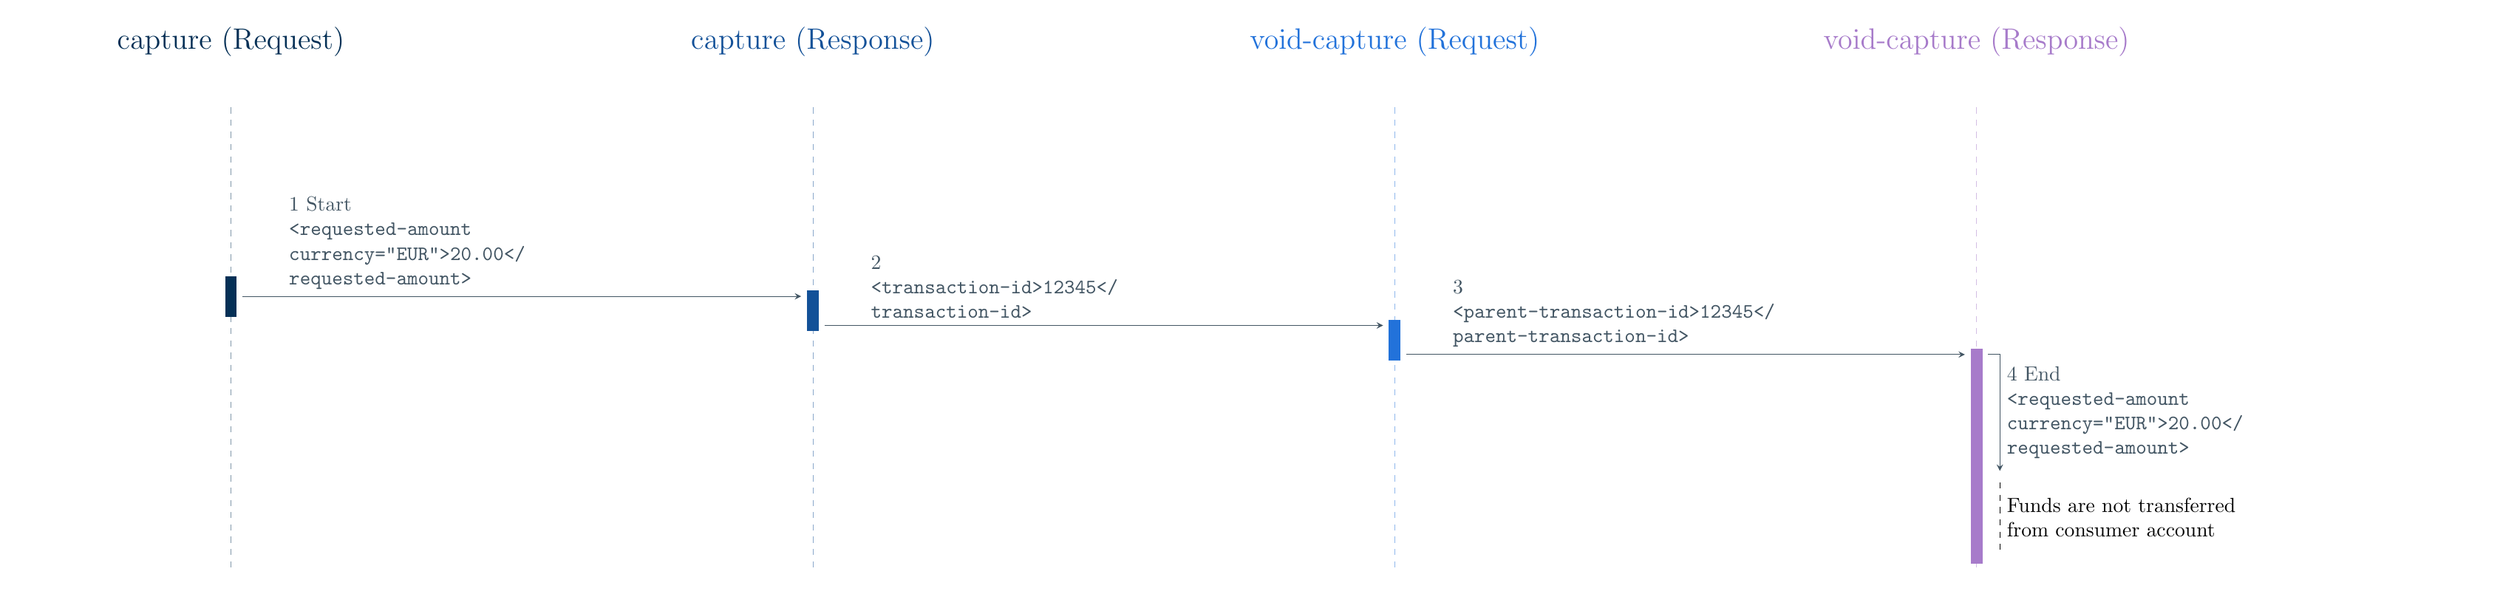
\begin{tikzpicture}

% Body
  % Participants
  \node[pt2] at (0,1.5) {capture (Request)};
   \node[pt3] at (10,1.5) {capture (Response)};
    \node[pt4] at (20,1.5) {void-capture (Request)};
     \node[pt1] at (30,1.5) {void-capture (Response)};
                      
 			 % Aid Lines
  			\draw[line_night] (0,0) -- (0,-8);
  			\draw[line_nightsky] (10,0) -- (10,-8);
 			\draw[line_sky] (20,0) -- (20,-8);
  			\draw[line_mulberry] (30,0) -- (30,-8);
  
                      % Nodes
                      \fill[night] (-0.1,-2.9) rectangle (0.1,-3.6);
                      \fill[nightsky] (9.9,-3.15) rectangle (10.1,-3.85);
                      \fill[sky] (19.9,-3.65) rectangle (20.1,-4.35);
                      \fill[mulberry] (29.9,-4.15) rectangle (30.1,-7.85);
                      
                      
                      % Arrows & Text
                      \draw[solidarrow, txt]
                      	(0.2,-3.25) -- node[midway,above] {1 Start \\ \texttt{<requested-amount \\ currency="EUR">20.00</ \\ requested-amount>}} (9.8,-3.25);
                      \draw[solidarrow, txt]
                      	(10.2,-3.75) -- node[midway,above] {2 \\ \texttt{<transaction-id>12345</ \\ transaction-id>}} (19.8,-3.75);
                      \draw[solidarrow, txt]
                      	(20.2,-4.25) -- node[midway,above] {3 \\ \texttt{<parent-transaction-id>12345</ \\ parent-transaction-id>}} (29.8,-4.25);
                      \draw[solidarrow, txt]
                      	(30.2,-4.25) -- (30.4,-4.25) -- node[midway,right] {4 End \\ \texttt{<requested-amount \\ currency="EUR">20.00</ \\ requested-amount>}} (30.4,-6.25);
                      		\draw[txt, dashed]
                      			(30.4,-6.45) -- node[midway,right] {Funds are not transferred \\ from consumer account} (30.4,-7.65);
                      
\end{tikzpicture}
\end{document}
